
%----------------------------------------------------------------------------------------
%	PACKAGES AND OTHER DOCUMENT CONFIGURATIONS
%----------------------------------------------------------------------------------------

\documentclass{article}

\usepackage{fancyhdr} % Required for custom headers
\usepackage{lastpage} % Required to determine the last page for the footer
\usepackage{extramarks} % Required for headers and footers
\usepackage{graphicx} % Required to insert images
\usepackage{mathtools, bm}
\usepackage{amssymb, bm}
\usepackage{graphicx}
\usepackage{float}
\usepackage{multirow}
\usepackage[table]{xcolor}  
\usepackage{algorithm}
\usepackage[noend]{algpseudocode}

% Margins
\topmargin=-0.45in
\evensidemargin=0in
\oddsidemargin=0in
\textwidth=6.5in
\textheight=9.0in
\headsep=0.25in


\linespread{1.1} % Line spacing

% Set up the header and footer
\pagestyle{fancy}
\lhead{\hmwkAuthorName} % Top left header
\chead{\hmwkTitleComp} % Top center header
\rhead{\firstxmark} % Top right header
\lfoot{\lastxmark} % Bottom left footer
\cfoot{} % Bottom center footer
\rfoot{Page\ \thepage\ of\ \pageref{LastPage}} % Bottom right footer
\renewcommand\headrulewidth{0.4pt} % Size of the header rule
\renewcommand\footrulewidth{0.4pt} % Size of the footer rule

\setlength\parindent{0pt} % Removes all indentation from paragraphs

%----------------------------------------------------------------------------------------
%	DOCUMENT STRUCTURE COMMANDS
%	Skip this unless you know what you're doing
%----------------------------------------------------------------------------------------

% Header and footer for when a page split occurs within a problem environment


% Header and footer for when a page split occurs between problem environments
   
%----------------------------------------------------------------------------------------
%	NAME AND CLASS SECTION
%----------------------------------------------------------------------------------------
\newcommand{\logoepfl}{
  \begin{center}
    
\includegraphics[width=4cm]{img/epfl.jpg}
  \end{center}
  \vspace{0.3cm}
  \hrule
}


\newcommand{\hmwkTitle}{Decentralized Verifiable Computation on Distributed Ledger}
\newcommand{\hmwkTitleComp}{Decentralized Verifiable Computation on Distributed Ledger} % Assignment title
\newcommand{\hmwkDueDate}{Summer 2018} % Due date
\newcommand{\hmwkClass}{IN, LCA1} % Course/class
\newcommand{\hmwkClassTime}{} % Class/lecture time
\newcommand{\hmwkClassInstructor}{D.Froelicher, J.Troncoso-Pastoriza} % Teacher/lecturer
\newcommand{\hmwkAuthorName}{Max Premi} % Your name

%----------------------------------------------------------------------------------------
%	TITLE PAGE
%----------------------------------------------------------------------------------------
\title{
\logoepfl
\vspace{2in}
\textmd{\textbf{\hmwkClass:\ \hmwkTitle}}\\
\normalsize\vspace{0.1in}\small{Due\ on\ \hmwkDueDate}\\
\vspace{0.1in}\large{\textit{\hmwkClassInstructor\ \hmwkClassTime}}
\author{\textbf{\hmwkAuthorName}}
\vspace{3in}
}

%----------------------------------------------------------------------------------------

\begin{document}

\maketitle

\newpage
\section*{Abstract}
\addcontentsline{toc}{section}{Abstract}
Data sharing systems are becoming more popular these past years, and are used in several domains, such as economics [REF], software validation [REF], and even in the medical field [REF]. They can be used for different purposes and might have goals that differ.\\
Eliminating singles point of failures is one of the central goal of decentralized systems,  but they can ensure the following properties: enforce transparency, provide an efficient way to ensure security, ensure authentication, and keep privacy of either parties and/or data.\\
The latter is required to respect privacy laws but introduces overhead such as encryption, verification of computation (\textit{correctness}), and tracking of error (\textit{robustness}).\\
UnLynx is such a system that uses Elliptic curve ElGamal encryption, zero-knowledge proof, and noise addition, as well as several other protocols to maintains all properties stated above. However, it only supports a small subset of operations (sum, count, average), and it has a strong threat model.\\
This project is a contribution to the design of a new decentralized system Lemal, supporting a large set of operations (mean, variance, logistic regression,...), while ensuring privacy and security in an efficient way, in addition of universal verifiability of computations and results.
In this project, we introduce a way to make all the proofs public and verifiable by anyone, through distributed ledger.
The goal of this project is to:
\begin{description}
\item[$\bullet$] First, propose a theoretical system implementation of the Skipchain, to create a Collective Authority of Verifying nodes (VNs) that guarantees correctness and robustness of computation.
\item[$\bullet$] Then, implement protocols that handle the Skipchain operations, based on the previous implementation done by DeDiS.
\item[$\bullet$] Implement the interface between the Collective authority doing the computation and the Collective authority of verifying nodes.
\item[$\bullet$] Finally, measure the performance of this system.
\end{description}

\newpage

\tableofcontents

\newpage

\section{Introduction}
Blockchain [REF] technology has emerged in 2008, with the Bitcoin, that uses distributed and decentralized ledger to create token and exchange them in a trusted way with immutability.
It has been widely popularized since 2008 with a total of 1604 cryptocurrencies [REF coinmarketcap] using different techniques of distributed ledger at the time of this report's writing.\\
However, its application can be extended to other topics, such as support for correctness and robustness of computations, as well as completely public zero-knowledge proofs.\\
Indeed, in a data sharing system, one of the biggest challenge is to ensure correctness without centralized authority.\\
Let's take the example of identity infrastructure. Nowadays, identity is proved trought cards that are issued by a central entity, the government. However, people are developping blockchain application to verify identity without central authority. Some challenges of this application would be to be be robust against classical attack, as well as provide result when ask for an identity and proof that it was correct (correctness).
Under certain threat model, it can be assumed that almost all parties are malicious, and it is needed to make a tremendous effort to prove that what has been done is correct. A distributed ledger can easily make a decentralized authority that can be consulted at any time to get data that were inserted and cannot be modified.\\
One of the major challenge is thus to handle the insertion of the data with a correct consensus, as well as the security of the protocol that interact with the ledger.\\
In this paper, we present the implementation of Skipchain [REF] into Lemal's framework, to deal with robustness and correctness of computation done by Lemal system. The chain will store information to verify the computation via zero-knowledge proof, without leaking anything more than what the proofs actually leak. Then a performance evaluation is done to look at the efficiency of such an implementation


\section{Contribution}
In this paper, the following contributions are made:\\
- A theoritical explanation of the design that will be used to make the VNs CA and skipchain secure, as well as robust an correct.\\


- An implementation of protocols to handle verification of proofs, and local storage of the later by the VNs.\\


- The deployment of a Skipchain using the previous implementation of DeDis as base, to store information about query verification by the verifying nodes as well as a way to retrieve all proof if one want to verify them.\\


- An evaluation of the performance in terms of efficiency and bandwidth, with a comparison to prior systems such as Unlynx.\\
\section{Background}
This section introduces some fundamental concepts used throughout the rest of the report. \textit{Collective Authority} that is the base of both system functionality. \textit{ElGamal encryption} is used in Lemal to ensure privacy, while \textit{Skiphain} is used in the verifying node as distributed Ledger. This section also introduces some fundamental background about Blockchain, as Skipchain is a structure derived from Blockchain.

\subsection{Collective Authority}
Nowadays, applications and systems rely on third-party authorities to provide security services. For example the creation of certificates to prove ownership of a public key. A collective authority is a set of $m$  servers that are deployed in a decentralized and distributed way, to support a given number of protocols.\\
Each of them possesses a private-public key pair $(k_i,K_i)$, where $K_i = k_i B$ with $k_i$ a scalar and $K_i$ a point in a given Elliptic Curve. This authority constructs a public key $K = \sum_{i=1}^{m}{K_i}$ which is the sum of all the server's public keys. To decrypt a message, each server $i$ partially decrypts a message encrypted using $k_{i}$. Thus the collective authority key provides strongest link security, as no intermediate can decrypt the data without the contribution of all the servers.

\subsection{ElGamal Encryption}
All the involved scalars belong to a field $\mathbb{Z}_p$.\\
For Unlynx, data are encrypted using Elliptic Curve ElGamal, more precisely, $P$ is a public key, $x$ is a message mapped to a point and $B$ is a base point on the curve $\gamma$. The encryption is the following, with $r$ a random nonce:\\
$E_P(x) = (rB,x+rP)$. The additive homomorphic property states that $\alpha E_P(x_1) + \beta E_P(x_2) = E_P(\alpha x_1+ \beta x_2)$\\
To decrypt, the owner of the private key $p$ satisfying $P = pB$ multiplies $rB$ and $p$ to get $rP$ and substracts it from $x + rP$ to recover $x$.\\

\subsection{Skipchain and Blockchain}
A blockchain is a continuously growing list of record (blocks), which are linked and secured using cryptographic functions. A block usually contains a hash of the previous block, a timestamp and data.\\
It is an open, distributed ledger recording block efficiently and that is verifiable and permanent.\\
A block is immutable and consensus between nodes is achieved with high Byzantine fault tolerance [REF].\\
A Skipchain is a mixed between blockchain and skiplist, meaning that the block contains forward and backward links, that can jump more than one block.\\


\section{Lemal System}
This section presents Lemal [REF] system in general. It goes through the system design, the assumptions made about the parties taking part in the different protocols, the properties that hold, and an example of a query that the system can handle.\\
\subsection{System Model}
\begin{figure}[H]
\center
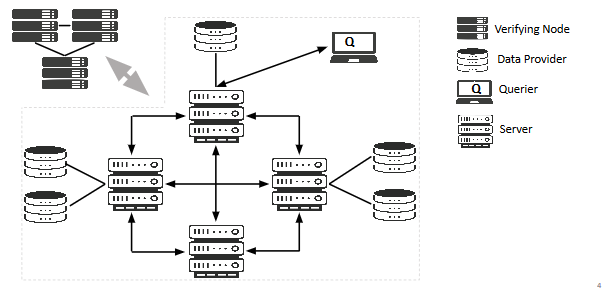
\includegraphics[scale=0.75]{img/lemal.png}
\caption{System model of Lemal}
\end{figure}
Lemal is a privacy-preserving data sharing system developed in collaboration of this project by LCA1. It consists of a collective authority (CA) formed by $m$ servers, $S_1,...S_m$ and $n$ data providers $DP_1,...DP_n$ containing sensitive data, encrypted using Elliptic Curve (EC) ElGamal.
Another collective authority of verifying nodes (VNs) is linked to this system and maintains a distributed ledger. It is described in Section 5. This system is used to answer queries made by a querier $Q$, to produce results of some aggregate functions. Each DP chooses one server of the CA to communicate with and can change this at any given time.\\
\textbf{Functionality}: Lemal permits a large set of SQL queries, like \textit{Where, group by, like, mean, variance, set intersection}, with some machine learning (\textit{linear and logistic regression}) and private recommender system functionality such as \textit{cosine similarity, CBF-Based recommendations, ...}.\\
For any query, proofs are computed and stored by verifying nodes in a Skipchain so that any party can verify what has been done.\\
\textbf{The pipeline} of the model is as follow:
\begin{itemize}
\item{Data providers send data with Range Proofs to CA server and verifying node}
\item{CA executes collective aggregation protocol and sends the proof to VNs}
\item{CA executes verifiable shuffling protocol and sends the proof to VNs}
\item{CA executes key switch protocol and sends the proof to VNs}
\item{VN did a probabilistic verification upon receiving proofs, the protocol to insert a block containing data to verify the query is launched}
\item{CA sends to querier its result}
\end{itemize}

\subsection{Threat Model}
\begin{figure}[H]
\center
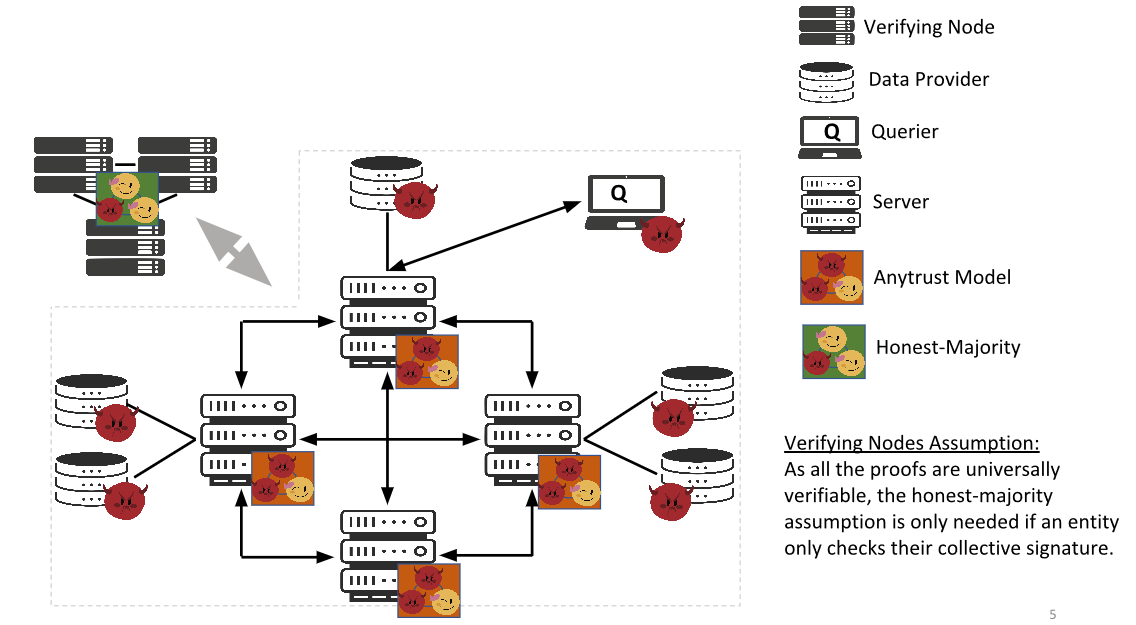
\includegraphics[scale=0.75]{img/threatLemal.png}
\caption{Threat model of Lemal}
\end{figure}
\textbf{Collective authority servers} It is assumed an Anytrust model [REF]. It does not require a particular server to be trusted or to be honest-but-curious. Whenever one of the servers is not malicious, functionality, security, and privacy are guaranteed.\\
\textbf{Collective authority verifying nodes} It assumes an Honest majority. Meaning a threshold of more than half of the nodes are honests, and the consensus is done via Byzantine fault tolerance protocol. This way, a consistent timeline is kept for the chain of blocks, and all data inserted on the chain are verified. Indeed, only one node of the VNs will start the insertion of data, that were collected from all the nodes, in the chain, so there is a verification function running on all node to verify that this node has not tried to insert  malicious data, but the one collected. This is different from the proof verification system, as we can insert value with proofs that were not valable to identify faulty parties in the proof verification. Here we ensure that the data inserted are coherent between the nodes of the VNs CA.\\
\textbf{The Querier, and Data providers} are assumed malicious. They can collude between themselves or with a subset of the CA servers.\\
It is also assumed that all network communication is encrypted and authenticated by using a protocol such as TLS or SSL.
\subsection{Properties}
\textbf{Confidentiality} All data are encrypted using EC ElGamal, no party sees the data in clear, except the Querier that get the aggregate result encrypted under his public key. This property holds as long as one server is honest.\\
\textbf{Privacy} The system ensures \textbf{differential privacy} for any individual sharing its data.\\
In all cases, the privacy of the querier is not addressed in this system, as we only care for the sensitive data of the DPs.\\
\textbf{Correctness} At each step of the protocol, zero-knowledge, non-interactive proofs are generated by the CA server or the DPs. These proofs can be used between two steps of the protocol to verify that computation was correctly done, and if it's not it can identify the entity that did not compute correctly.\\
\textbf{Robustness} is assured through the distributed ledger. In case of faulty computation, the block contains the verification of proof at each server.
If there is an incoherence in this verifications, the block also contains all the proofs for this query by the way of a link to a file.\\
Anyone can verify and identify the server/DP or a set of them that cheated.\\
This way, one could exclude these malicious parties from the protocol.

\subsection{Query example}
This subsection details the pipeline of a query process.\\
First, the querier $Q$ send a query to the CA server. The example taken in this section is "SELECT average(x) FROM y WHERE y.z $< 321$".\\
This query is received by a server $s$ of the CA and broadcasted to the entire CA. Then each server sends to its DPs, the query. The DPs execute it locally, then send the result encrypted with the CA's public key to each server that sends them the query.\\
The first proof is sent with each data, proving that the cipher resulting from each DP is in a given range.\\
At this point, each server of the CA contains ciphers encrypted with the CA's public key.
Then, a collective aggregation is done. In the current example, the server will add the ciphers and the root server (the one the querier contacted) will initiate an aggregation protocol, to get all the final result, which is the sum at each server and the number of values. This protocol is done with a tree implementation. Children servers will send their average to their parent, it will aggregate, and the same thing will happen until the top of the tree is reached.\\
Again, a proof is generated, which is just the cipher before and after aggregation.\\
At this point, there might be differential privacy applied to perturb end-result in order to satisfy privacy. In this example, servers might collectively add several time values that does not make the whole mean varies too much, but it gives privacy on the number of values, and individual result at each server.\\
This comes from Unlynx with Distributed Results Obfuscation (DRO) step, that enables the CA to collectively and homomorphically add noise, sampled form a probabilistic distribution.
To do so, a shuffling phase is initiated, where multiple sequences of noise are randomly permutated. This ensures that the noise is randomly chosen for a given querry.\\
The shuffle is also verifiable, a proof is generated at each server when its execution is finished.\\
Finally, a key switch protocol is engaged. It permits to sequentially add values to the final result to finish with a cipher encrypted under the public key of the querier. To do so, each server adds an element containing a nonce and its public key, with the proof of what it computed is correct.\\
Eventually, the root server sends back the result to the querier.\\


Note that we did not include the Verifying nodes process in this query example as we detail it further in the following section.

\section{Verifying  Node}
This section presents the implementation of the Verifying nodes CA. It was the main goal of this project and will be the major part of this report. We will first present in details the threat model and the theoretical system model, then the operations supported, and in the following section the way we choose to implement it.\\
\subsection{System Model}
The verifying node CA's goal is to relax the proof verification time of potential client, by doing the computations, and store it inside a block of a distributed ledger.\\
To avoid taking a long time to verify all the proofs, several modifications are done.\\
First, when a query is received by the CA, the exact number of proof expected for each type is known. So the CA sends to the VNs this number to initialize a dictionary that will be refered as "\textit{bitmap}" from now on.\\
Then, proofs are sent as soon as they are created to all nodes of the VNs CA. Each of them verifies a set of the proof chosen probabilistically with a fixed threshold $p \in (0,1]$. Each server chose the subset in a uniform way, so the sets are different with high probability, and might intersect.\\
It results in a $1$ if the proof is correct, $0$ if incorrect and $2$ if it has not been verified.\\
To be sure that the proof are coming from the correct entity, all of them are signed by the server/DP that issued it.\\
After verifying these proofs, it stores the result of the verification in the dictionary (bitmap) with the name of the server and the proof's hash as key and the verification result as value in a local database. The proofs are also store in this database.\\
So when a proof $p$ is received by a node of the VNs, it randomly verify it, and store $2$ values:\\
bitmap[\textit{serverID+hash($p$)}] = verif($p$), this bitmap is saved in the local database for each query, and will be stored in the Skipchain.\\
(\textit{queryID},$p$) is also stored in the local database, but will be kept after the query is finished.
It then waits for other proof of the same query to be received, and does the same for all other types of proofs.\\
Upon receiving the last proofs, i.e. when the bitmap has been entirely filled, each server gather all results of verification inside a unique bitmap, and a protocol to gather all bitmap to one root server is launched.\\
At the end of this protocol, the root server launches an insert (or a create chain if there is none yet) block operation given the bitmap aggregated, the name of the file containing all the proofs, and a timestamp.\\
If the block is correctly inserted, and the automatic verification is done by each server pass, then it inserts the block, else it will not insert it. In this case, the verification done by each server is checking whether its bitmap appears in the data of the new block request. If it does not appear it means a fraudulent server tried to falsify information.\\
Any client can fetch the last block of the Skipchain at any time.

\subsection{Threat Model}
As described previously, the threat model of the VNs CA is Honest-majority. This means that at least half of the server are honest. This properties must hold in order to maintain the Skipchain correctly.

\subsection{Type of Proof}
As described in section 4.4, the CA server generates a different kind of proofs. This subsection will present in details what they contain and how they are verified. All these proofs come from Unlynx [REF] framework.\\
\textbf{Range proofs} are computed by each DP. They prove that a commitment $C$ is in a range $[a,b]$. This is used to handle malicious DP input. In a query with range predicate, it is perfect to prove that an encrypted data indeed lies in a given range, without leaking the value in itself. This proof was designed to compare Prio and Unlynx in a previous project [REF].\\
\textbf{Shuffle proofs} are computed by the CA server to prove privacy. This ensures the privacy of previously verified data, with differential privacy via noise addition.\\
\textbf{Aggregation proofs} are also computed by the CA server. It ensures correctness of computation, without leaking any information on data, except the information that the operation leaks in itself. For example, a mean operation will leak the number of data that the CA aggregates.\\
\textbf{Key Switch proofs} are computed by the CA server. These proofs ensure the security of data, and correctness of computations. Its goal is to verify that the protocol to switch encryption key is correct without leaking the data in clear.\\

\subsection{Operations supported}
Here, the operations supported by the verifying node are presented in details.\\
There are two services that we can distinguish. The first one is the service that handles the proofs receiving, verification and storage.\\
The other service handles the communication with the Skipchain, as well as the function and data accepted by the Skipchain.\\ 
\section{Implementation}
In this section, the technical implementation of the VNs CA is detailed. All the implementation was done in Unlynx branch called Lemal [REF].\\
We first present the service that handles, verify and store the proofs. Then the service that handles the communication with the Skipchain.\\
Finally, the modification made to the Skipchain service of DeDiS [REF] is addressed in the last part.
\section{Performance Evaluation}
\section{Conclusion and Future Work}
\begin{thebibliography}{9}
\bibitem{prioimple}
Henry Corrigan-Gibbs, Prio prototype implementation\\
\texttt{https://github.com/henrycg/prio}
\end{thebibliography}
\end{document}
